% !TEX root = ../../../main.tex
% 来源：中学数学实验教材·第三册（高中数学）
% 章节：不等式和解不等式 / 解不等式
% 原始文件：3.tex，行 2050-2098
% 类型：tikz
% ---
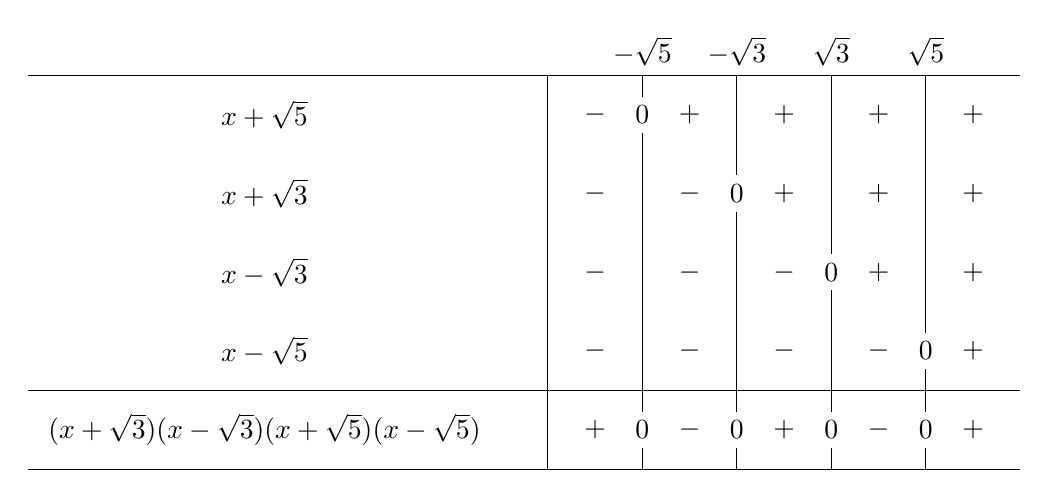
\begin{tikzpicture}[yscale=2, xscale=1.2]
\foreach \x in {0,.5,2.5}
{
    \draw (0,\x)--(10.5,\x);
}
\foreach \x/\xtext in {5.5/{},6.5/-\sqrt{5},7.5/-\sqrt{3},8.5/\sqrt{3},9.5/\sqrt{5}}
{
    \draw (\x,0)--(\x,2.5)node[above]{$\xtext$};
}

\node at (2.5,.25){$(x+\sqrt{3})(x-\sqrt{3})(x+\sqrt{5})(x-\sqrt{5})$};
\foreach \x/\xtext in {6/+,7/-,8/+,9/-,10/+}
{
    \node at (\x,.25) {$\xtext$};
}

\node at (2.5,.75){$x-\sqrt{5}$};
\foreach \x/\xtext in {6/-,7/-,8/-,9/-,10/+}
{
    \node at (\x,.75) {$\xtext$};
}

\node at (2.5,1.25){$x-\sqrt{3}$};
\foreach \x/\xtext in {6/-,7/-,8/-,9/+,10/+}
{
    \node at (\x,1.25) {$\xtext$};
}

\node at (2.5,1.75){$x+\sqrt{3}$};
\foreach \x/\xtext in {6/-,7/-,8/+,9/+,10/+}
{
    \node at (\x,1.75) {$\xtext$};
}

\node at (2.5,2.25){$x+\sqrt{5}$};
\foreach \x/\xtext in {6/-,7/+,8/+,9/+,10/+}
{
    \node at (\x,2.25) {$\xtext$};
}

\foreach \x in {6.5,7.5,8.5,9.5}
{
    \node at (\x,.25)[fill=white] {0};
}
\node at (9.5,.75)[fill=white] {0};
\node at (7.5,1.75)[fill=white] {0};
\node at (6.5,2.25)[fill=white] {0};
\node at (8.5,1.25)[fill=white] {0};
\end{tikzpicture}
